\documentclass[a4paper,12pt]{report}
\usepackage{geometry} % Для последующего задания полей
\geometry{a4paper,top=15mm,bottom=20mm,left=10mm,right=10mm}
\usepackage[T2A]{fontenc}	     % Поддержка русских букв
\usepackage[utf8]{inputenc}	     % Кодировка utf8
\usepackage[english, russian]{babel} % Языки: русский, английский
\usepackage{graphicx}                % Подключаем пакет работы с графикой

\renewcommand{\arraystretch}{1.3}

\begin{document}


\section*{Исходные данные}

\begin{table}[h!]
  \renewcommand{\tabcolsep}{0.9em}
  \centering
  \begin{tabular}{cccccccccc}
    -4.86	& -3.7	& -2.41	& -2.24	& -2.12	& -2.07	& -1.87	& -1.57	& -1.05	& -0.95	\\ 
-0.86	& -0.82	& -0.69	& -0.56	& -0.42	& -0.38	& -0.14	& -0.13	& -0.01	& 0.1	\\ 
0.13	& 0.41	& 0.46	& 0.53	& 0.7	& 0.84	& 0.99	& 1.06	& 1.19	& 1.21	\\ 
1.21	& 1.21	& 1.23	& 1.26	& 1.33	& 1.47	& 1.76	& 1.91	& 1.94	& 2.02	\\ 
2.09	& 2.12	& 2.2	& 2.22	& 2.24	& 2.37	& 2.38	& 2.45	& 2.51	& 2.6	\\ 
2.6	& 2.65	& 2.67	& 2.69	& 2.88	& 3.12	& 3.15	& 3.23	& 3.24	& 3.24	\\ 
3.26	& 3.44	& 4.09	& 4.09	& 4.47	& 4.79	& 4.95	& 5.01	& 5.03	& 5.18	\\ 
5.2	& 5.21	& 5.36	& 5.44	& 5.44	& 5.47	& 5.48	& 5.64	& 5.78	& 5.79	\\ 
5.81	& 5.94	& 5.98	& 6.11	& 6.49	& 6.54	& 6.63	& 6.75	& 7.05	& 7.13	\\ 
7.17	& 7.34	& 7.51	& 7.85	& 7.93	& 8.7	& 9.26	& 9.5	& 10.95	& 11.15	\\ 
	\\ 

  \end{tabular}
  \caption{Исходная выборка}
\end{table}

\section*{Линия регрессии}

\begin{figure}[h!] 
  \centering
  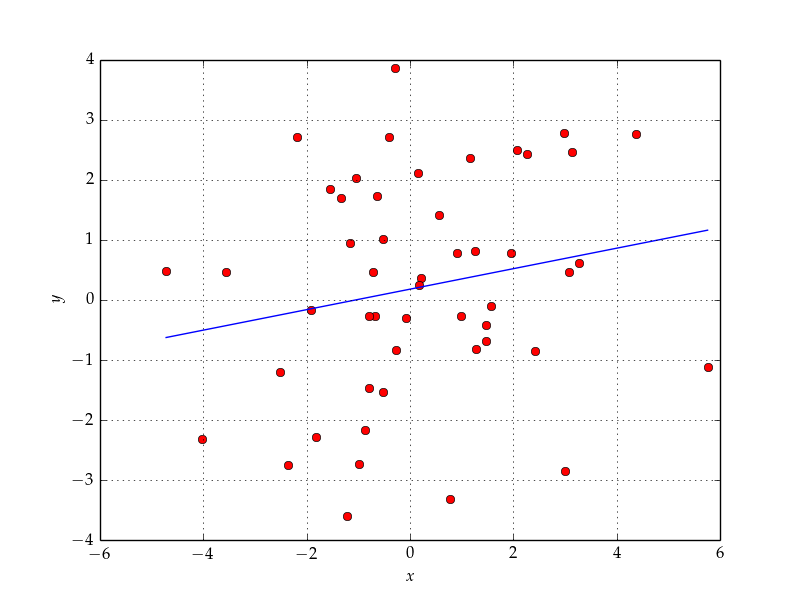
\includegraphics[width=0.8\linewidth]{../pic/sample_regression}
  \caption{График линии регрессии для заданной выборки}
\end{figure}


\end{document}